% =============================================================================
% slides.tex — UGP presentation (about 10 minutes).
% Theme: Midcentury Modern by Jules Leguy (CC BY 4.0),
%        https://github.com/jules-leguy/midcenturymodern
% Build: tectonic slides.tex    (or LuaLaTeX on Overleaf)
% =============================================================================
\documentclass[aspectratio=169]{beamer}
\usepackage{beamerthememidcenturymodern}
\usepackage{booktabs}
\mcmTheme{Kraft}

\title{Natural Language Path Finding}
\subtitle{Walkable paths, from everyday instructions}
\author{Shashi Bhidodiya \and Krishna Kumayu}
\institute{Supervisor: Prof.\ Indranil Saha \\ Dept.\ of CSE, IIT Kanpur}
\date{Undergraduate Project}

\AtBeginSection[]{%
  \begin{frame}[plain]
    \sectionpage
  \end{frame}
}

\newcommand{\nopath}{\texttt{NO\_PATH}}

\begin{document}

% -----------------------------------------------------------------------------
\begin{frame}
  \titlepage
\end{frame}

% =============================================================================
\section{The Problem}
% =============================================================================

\begin{frame}{What do people actually say?}
  \begin{center}
    \large
    ``Go to the \alert{lab}, don't go through the \alert{workshop},\\
    stop at the \alert{store room} first, and stay in the \alert{corridor}
    if you can.''
  \end{center}
  \vspace{1em}
  \begin{columns}[T]
    \begin{column}{0.23\textwidth}
      \begin{block}{Goal}
        go to the lab
      \end{block}
    \end{column}
    \begin{column}{0.23\textwidth}
      \begin{block}{Never}
        not the workshop
      \end{block}
    \end{column}
    \begin{column}{0.23\textwidth}
      \begin{block}{In order}
        store room first
      \end{block}
    \end{column}
    \begin{column}{0.23\textwidth}
      \begin{block}{If you can}
        prefer the corridor
      \end{block}
    \end{column}
  \end{columns}
  \vspace{1em}
  A normal path planner (A*) only understands \textbf{one goal cell}.
\end{frame}

\begin{frame}{Two existing ways, and both have a problem}
  \begin{columns}[T]
    \begin{column}{0.48\textwidth}
      \begin{alertblock}{1. Ask the LLM for the path}
        \begin{itemize}
          \item The LLM reads the map and writes the cells
          \item Understands any sentence
          \item[] \textbf{But:} nothing stops it from walking
            \textbf{through walls}
        \end{itemize}
      \end{alertblock}
    \end{column}
    \begin{column}{0.48\textwidth}
      \begin{alertblock}{2. Translate to a logic formula}
        \begin{itemize}
          \item LLM writes a formula (LTL), a planner follows it
          \item Correct \emph{if} the formula is correct
          \item[] \textbf{But:} formulas are \textbf{easy to get wrong},
            hard to read, and cannot say ``if you can''
        \end{itemize}
      \end{alertblock}
    \end{column}
  \end{columns}
  \vspace{1em}
  \begin{center}
    We want: \textbf{any sentence} in, a \textbf{safe and correct path} out.
  \end{center}
\end{frame}

% =============================================================================
\section{Our Idea}
% =============================================================================

\begin{frame}{The LLM decides \emph{what}, A* decides \emph{how}}
  \begin{columns}[c]
    \begin{column}{0.48\textwidth}
      The LLM only fills a small form.\\
      It \textbf{never sees the map} and never writes a cell.
      \vspace{0.8em}
      \begin{exampleblock}{Intent form (from the sentence)}
        \small
        \begin{tabular}{@{}ll}
          goal      & lab \\
          forbidden & workshop \\
          stops     & store room \\
          prefer    & corridor \\
          avoid     & --- \\
        \end{tabular}
      \end{exampleblock}
    \end{column}
    \begin{column}{0.48\textwidth}
      \begin{block}{Why a form?}
        \begin{itemize}
          \item Easy for the LLM to fill
          \item Easy for a person to read and check
          \item Can say ``if you can''
          \item Wrong names are caught and sent back
            (at most 3 tries)
        \end{itemize}
      \end{block}
    \end{column}
  \end{columns}
\end{frame}

\begin{frame}{The pipeline}
  \centering
  \begin{tikzpicture}[
      box/.style={draw=mcmPrimary, line width=0.8pt, rounded corners=3pt,
                  align=center, minimum height=1.3cm, text width=2.5cm,
                  font=\small},
      arr/.style={-latex, line width=1pt, draw=mcmPrimary}]
    \node[box, fill=mcmAlert!25] (p) at (0,0)   {\textbf{1. Parser}\\LLM fills\\the form};
    \node[box] (c) at (3.4,0)  {\textbf{2. Compiler}\\form $\to$ walls\\and costs};
    \node[box] (a) at (6.8,0)  {\textbf{3. Planner}\\A* finds the\\cheapest path};
    \node[box] (v) at (10.2,0) {\textbf{4. Checker}\\re-checks\\every path};
    \draw[arr] (p) -- (c);
    \draw[arr] (c) -- (a);
    \draw[arr] (a) -- (v);
  \end{tikzpicture}

  \vspace{1.5em}
  \begin{columns}[T]
    \begin{column}{0.30\textwidth}
      \textbf{Forbidden} room\\ $\to$ becomes a wall
    \end{column}
    \begin{column}{0.30\textwidth}
      \textbf{Prefer} = cheaper (0.5)\\
      \textbf{Avoid} = costlier (3)
    \end{column}
    \begin{column}{0.30\textwidth}
      \textbf{Stops in order}\\ $\to$ planner counts the\\ stops done so far
    \end{column}
  \end{columns}
\end{frame}

\begin{frame}{What we can guarantee}
  \framesubtitle{Proved on paper, and tested on 1000s of random maps}
  \begin{enumerate}
    \item The path is \textbf{always walkable}, even if the LLM misunderstood
      the sentence.
    \item It follows every rule in the form (never, in order, goal).
    \item If we say \nopath, then \textbf{no path exists}.
    \item It is the \textbf{cheapest} such path.
    \item ``If you can'' never causes a huge detour (bounded).
  \end{enumerate}
  \vspace{0.8em}
  \begin{alertblock}{What is \emph{not} guaranteed}
    That the LLM reads the sentence correctly, so we \textbf{measure} it.
  \end{alertblock}
\end{frame}

% =============================================================================
\section{Experiments}
% =============================================================================

\begin{frame}{Setup}
  \begin{columns}[T]
    \begin{column}{0.48\textwidth}
      \begin{block}{Benchmark}
        \begin{itemize}
          \item 20 generated floor plans (40 × 40 grid)
          \item 165 instructions, each in \textbf{3 wordings} = 495
          \item Types: plain, never, stop, in order, ``if you can'', impossible
          \item 30 written by hand, deliberately messy
        \end{itemize}
      \end{block}
    \end{column}
    \begin{column}{0.48\textwidth}
      \begin{block}{Methods compared}
        \begin{itemize}
          \item \textbf{M0} plain A* (ignores the rules)
          \item \textbf{M1} LLM writes the path
          \item \textbf{M2} LLM writes a logic formula
          \item \textbf{M3} ours (intent form)
        \end{itemize}
        Same LLM for all: Google Gemini
      \end{block}
    \end{column}
  \end{columns}
\end{frame}

\begin{frame}{Main result}
  \begin{columns}[c]
    \begin{column}{0.55\textwidth}
      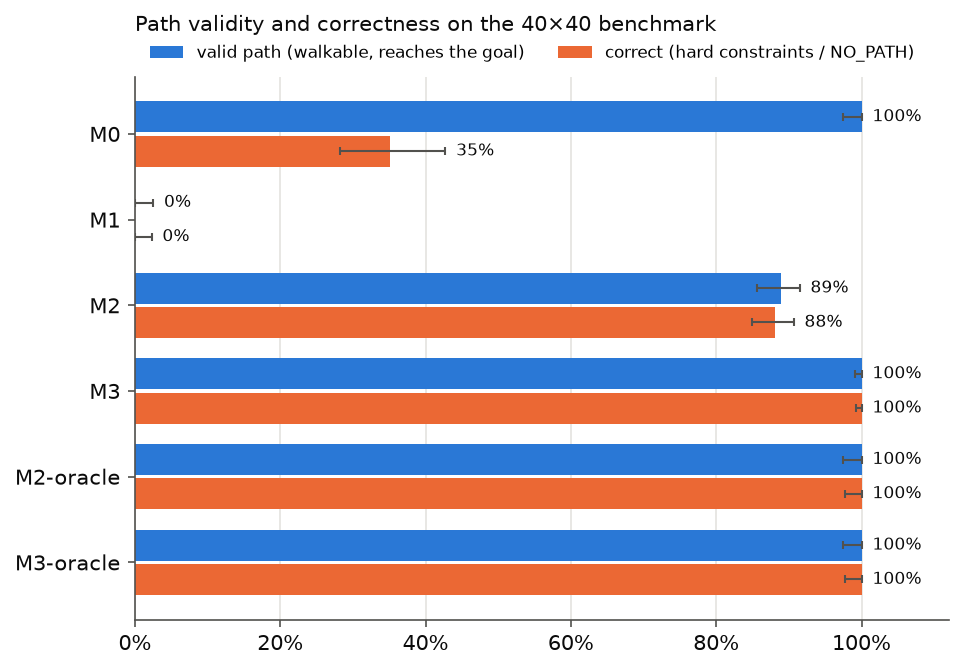
\includegraphics[width=\textwidth]{figures/validity.png}
    \end{column}
    \begin{column}{0.42\textwidth}
      \begin{tabular}{@{}lr@{}}
        \toprule
        Method & Correct \\
        \midrule
        M0 plain A* & 35\% \\
        M1 LLM writes path & 0\% \\
        M2 logic formula & 88\% \\
        \textbf{M3 ours} & \textbf{100\%} \\
        \bottomrule
      \end{tabular}
      \vspace{1em}

      On ``in order'' instructions the formula method is right only
      \textbf{61\%} of the time.

      \vspace{0.6em}
      {\small \textit{Oracle} = the planner is given the correct form /
      formula directly (no LLM).}
    \end{column}
  \end{columns}
\end{frame}

\begin{frame}{LLM writing the path: through the walls}
  \centering
  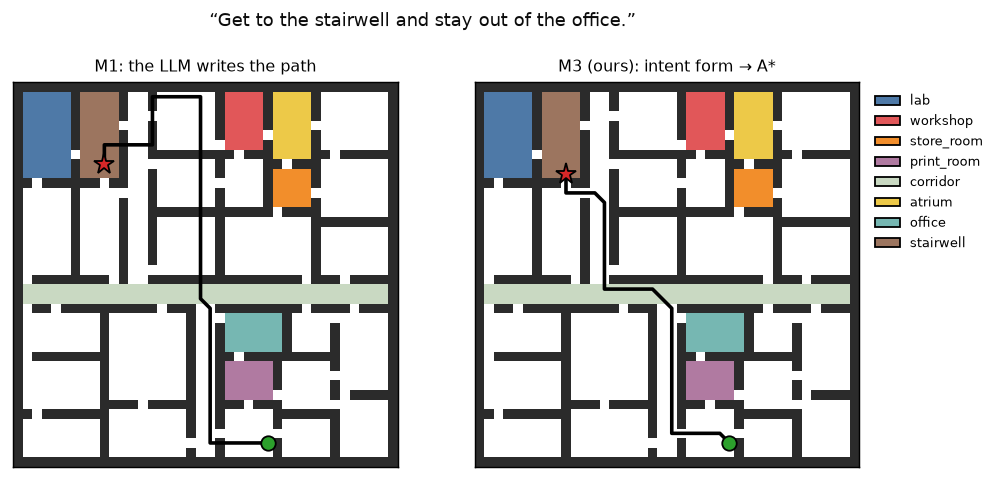
\includegraphics[width=0.78\textwidth]{figures/m1_vs_m3.png}

  \vspace{0.3em}
  160 of 161 LLM-written paths were \textbf{not walkable}.
  Ours: all walkable.
\end{frame}

\begin{frame}{Why does the formula method lose?}
  \begin{columns}[T]
    \begin{column}{0.5\textwidth}
      \begin{tabular}{@{}lcc@{}}
        \toprule
        & Form & Formula \\
        \midrule
        LLM got it right & \textbf{100\%} & 56\% \\
        Same for all 3 wordings & \textbf{100\%} & 30\% \\
        \bottomrule
      \end{tabular}
    \end{column}
    \begin{column}{0.46\textwidth}
      \begin{block}{In short}
        \begin{itemize}
          \item Both planners are perfect when given the right input
          \item So the loss is in the \textbf{LLM's translation}
          \item Filling a form is much easier than writing logic
        \end{itemize}
      \end{block}
    \end{column}
  \end{columns}
\end{frame}

\begin{frame}{``If you can'': only the form can trade off}
  \centering
  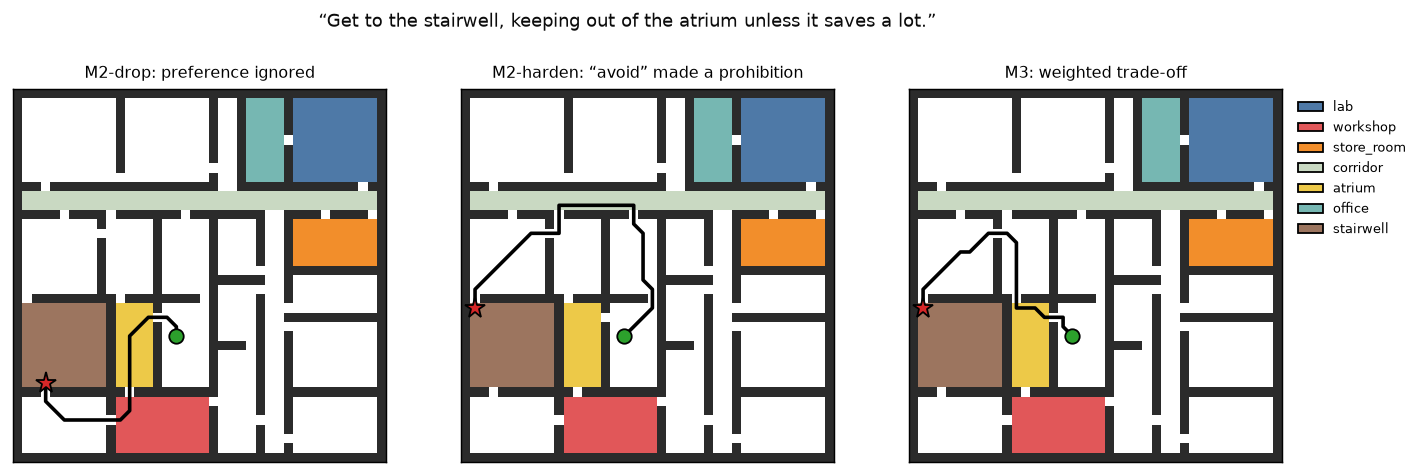
\includegraphics[width=0.9\textwidth]{figures/soft_harden.png}

  \vspace{0.2em}
  \small
  Ignore it (left) $\cdot$ make it a strict rule, long detour (middle)
  $\cdot$ \textbf{ours: balanced} (right)\\
  Ours spends about \textbf{twice as much} of the path in the preferred
  corridor, for paths only \textbf{9\%} longer on average.
\end{frame}

% =============================================================================
\section{Next Steps}
% =============================================================================

\begin{frame}{Limitations}
  \begin{itemize}
    \item The LLM's reading is not guaranteed, only measured
    \item Benchmark is generated: short sentences, known room names
    \item One LLM (Gemini Flash-Lite) tested
    \item Not yet tested with a real robot
    \item M1 and M2 are \textbf{our own versions} of the two approaches,
      not the published systems
  \end{itemize}
\end{frame}

\begin{frame}{Future work}
  \begin{columns}[T]
    \begin{column}{0.48\textwidth}
      \begin{block}{Compare with published LLM planners}
        \begin{itemize}
          \item \textbf{LLM-A*}: LLM suggests waypoints, A* joins them
          \item \textbf{LLM+P}: LLM writes a problem for a classical planner
          \item Published NL-to-logic systems
        \end{itemize}
      \end{block}
    \end{column}
    \begin{column}{0.48\textwidth}
      \begin{block}{Make it more realistic}
        \begin{itemize}
          \item Real building maps and real people's instructions
          \item \textbf{ROS/Gazebo simulation}: a simulated robot follows
            our paths (needed for publication)
          \item Then test on a real mobile robot
        \end{itemize}
      \end{block}
    \end{column}
  \end{columns}
  % \begin{columns}[T]
  %   \begin{column}{0.48\textwidth}
  %     \begin{block}{Compare with published LLM planners}
  %       \begin{itemize}
  %         \item \textbf{LLM-A*}: LLM suggests waypoints, A* joins them
  %         \item \textbf{LLM+P}: LLM writes a problem for a classical planner
  %         \item Published NL-to-logic systems
  %       \end{itemize}
  %     \end{block}
  %     \begin{block}{Make it more realistic}
  %       \begin{itemize}
  %         \item Real building maps, real people's instructions
  %         \item Try on a mobile robot
  %       \end{itemize}
  %     \end{block}
  %   \end{column}
  %   % \begin{column}{0.48\textwidth}
  %   %   \begin{exampleblock}{Target: IROS 2027}
  %   %     Paper deadline \textbf{1 March 2027} (tentative)
  %   %     \vspace{0.4em}
  %   %     \begin{itemize}
  %   %       \item Dec--Jan: add new comparisons
  %   %       \item Jan: write the paper
  %   %       \item Feb: review with Prof.\ Saha
  %   %       \item 1 Mar: submit
  %   %     \end{itemize}
  %   %   \end{exampleblock}
  %   %   Report already prepared in IROS format.
  %   % \end{column}
  % \end{columns}
\end{frame}

% \begin{frame}{Summary}
%   \begin{itemize}
%     \item Let the LLM \textbf{understand}, let A* \textbf{plan}
%     \item Paths are \textbf{always walkable} and follow the rules
%     \item 100\% correct vs 88\% (formula) and 0\% (LLM writes path)
%     \item Handles ``if you can'' with a small, bounded detour
%   \end{itemize}
% \end{frame}

% -----------------------------------------------------------------------------
{\setbeamercolor{normal text}{fg=mcmPrimaryFg,bg=mcmAlert!70}
\begin{frame}[plain,noframenumbering]
  \begin{center}
    \Large
    Thank you!\\[0.5em]
  \end{center}
\end{frame}
}

\end{document}
